%
% Latex document for paper ``Why Do the Rich Save So Much?''
%

\documentclass[titlepage,12pt]{article}
\usepackage{ifthen,minted,natbib,amsmath}

\newboolean{Figures}
\setboolean{Figures}{true}

\newboolean{PublicationVersion}
\setboolean{PublicationVersion}{false}

\usepackage{ushort}
\usepackage{graphicx}
\usepackage{hyperref}

\begin{document}
      

\begin{titlepage}
%\hfill Final Version

%\vspace{.75in}
{\centerline {\LARGE Why Do the Rich Save So Much?}}
\vspace{0.5in}


\centerline{Christopher D. Carroll}
\centerline{The Johns Hopkins University}
\centerline{ccarroll@jhu.edu}

\medskip\medskip


\centerline{November 3, 2000}


\vspace{0.1in}

\centerline{\bf Abstract}

This paper considers several alternative explanations for the fact 
that households with higher levels of lifetime income (`the rich') 
have higher lifetime saving rates (Dynan, Skinner, and 
Zeldes~\citeyear{dsz:richsave}; Lillard and 
Karoly~\citeyear{lillard&karoly:richsave}).  The paper argues that the 
saving behavior of the richest households cannot be explained by 
models in which the only purpose of wealth accumulation is to finance 
future consumption, either their own or that of heirs.  The paper 
concludes that the simplest model that explains the relevant facts is 
one in which either consumers regard the accumulation of wealth as an 
end in itself, or unspent wealth yields a flow of services (such as 
power or social status) which have the same practical effect on 
behavior as if wealth were intrinsically desirable.

\vspace{.2in}
\noindent {\bf Keywords:} saving, consumption, Life Cycle model, rich, 
bequests, inheritance

\medskip
\noindent {\bf JEL Codes:} D11, D12, D31, D91, E21 H23, H24 

\medskip \medskip This paper was published in the volume {\it Does Atlas Shrug?
The Economic Consequences of Taxing the Rich}, Harvard University Press, 
2000, Edited by Joel B. Slemrod:

\begin{tiny}
\begin{minted}{latex}
@inproceedings{WhyDoTheRich,
  author = {Christopher D. Carroll},
  booktitle = {Does Atlas Shrug? The Economic Consequences of Taxing the Rich},
  editor = {Joel B. Slemrod},
  publisher = {Harvard University Press},
  title = {Why Do the Rich Save So Much?},
  chapter = 14,
  year = 2000,
  url = {https://llorracc.github.com/WhyDoTheRich/blob/main/Why.pdf},
}
\end{minted}
\end{tiny}

{\small I am indebted to Sidney Carroll, Elizabeth B. 
Carroll, and Elizabeth I. Carroll for many of the insights in this 
paper.  Any errors are my own.}

\end{titlepage}

\baselineskip 22pt
\vspace{0.5in}
\ifthenelse{\boolean{PublicationVersion}}{
\addtolength{\footnotesep}{5pt}
\baselineskip 30pt
}

\begin{quote}
\noindent F. Scott Fitzgerald, to Ernest Hemingway: \newline
\indent	{~~~~}``The very rich are different from you and me.''
	

\noindent Ernest Hemingway, to F. Scott Fitzgerald: \newline \indent 
\indent {~~~~}``Yes.  They have more money.''\footnote{This is a paraphrase of a 
conversation cited in {\it Bartlett's Familiar 
  Quotations}~\citeyear{bartlett:quotes}}
\end{quote}

\hypertarget{introduction}{}
\section{Introduction}

The saving behavior of the wealthy has received remarkably little 
academic attention in the past twenty years or so.  This is probably 
largely attributable to a relative lack of good data: The {\it Survey 
of Consumer Finances} is virtually the only publicly available source 
of detailed data on wealthy households, and even the SCF has only a 
few hundred really wealthy households in each triennial wave.  Despite 
recent neglect, the topic is an important one for scholars of saving 
behavior, for at least two reasons.  First, wealthy households should 
provide a powerful means of testing whether the standard model of 
consumer behavior, the Life Cycle/Permanent Income Hypothesis, is 
adequate as a universal model of saving and consumption.  This is an 
application of the general scientific principle that models should be 
tested under extreme conditions; if they do not hold up, a new model 
(or an extended version of the old one) is called for.  The second 
reason for studying the wealthy is that they account for a large share 
of aggregate wealth.  In fact, some understanding of the saving 
behavior of the wealthy is probably indispensable to any credible 
attempt to account for the magnitude of aggregate wealth.

Although the primary source of evidence in this paper will be the four 
{\it Surveys of Consumer Finances} conducted in 1983, 1989, 1992, and 
1995, the inevitable limitations of those data will be apparent.  The 
paper therefore also relies to a considerable extent on unorthodox 
kinds of evidence, ranging from information in the annual {\it Forbes 
400} tabulation of the richest American households, to quotations from and 
about the very rich, to the results of a ``focus group'' meeting with 
a set of wealthy individuals who were directly asked their reasons for 
saving.

The paper begins by considering whether the standard model of 
household consumption and saving decisions, the Life Cycle model, 
provides an adequate description of the behavior of wealthy 
households.  I argue that the Life Cycle model, or at least the 
traditional incarnation in which the decision-maker saves mainly to 
finance his own future consumption, cannot simultaneously explain both 
the behavior of the median household and the behavior in the 
upper tail of the wealth distribution.  The next section of the paper 
considers whether a ``Dynastic'' model, in which the wealthy save 
mainly for the benefit of their heirs, performs better.  While the 
Dynastic model can explain some observations, and probably does 
roughly apply to some households, I argue that it still does not 
explain some important facts about the saving behavior of the wealthy.  
Furthermore, the Dynastic model conflicts with the self-reported 
motives for saving that many wealthy people voice.  Finally, I 
consider a model in which the wealthy save because, either directly or 
indirectly, they obtain greater pleasure from possessing an extra 
dollar of wealth than they would get from an extra dollar of 
consumption.  Following Max Weber~\citeyear{weber:capitalism} as 
interpreted by Zou~\citeyear{zou:spirit} and Bakshi and 
Chen~\citeyear{bakshi&chen:spirit}, I call this the ``Capitalist Spirit'' 
model.  I argue that a direct wealth accumulation motive is 
indispensable in explaining at least some of the observed behavior of 
the very wealthy.

\hypertarget{can-the-life-cycle-model-explain-the-behavior-of-the-wealthy}{}
\section{Can the Life Cycle Model Explain the Behavior of the Wealthy?}
\label{sec:LCModel}
A provocative recent paper by Hubbard, Skinner, and 
Zeldes~\citeyear{hsz:importance} (henceforth, HSZ) argues that an expanded 
version of the Life Cycle model in which uncertainty is modelled 
realistically can generate patterns of wealth accumulation that are 
roughly consistent with average data from household surveys, and 
amounts of aggregate wealth that are similar to observed aggregate 
household wealth in the U.S. If such a model really did produce 
roughly correct predictions for household wealth holdings, there would 
be little need to study the very wealthy in detail, since they would 
merely be scaled-up versions of everyone else.

Behind the scenes of the HSZ model, however, all is not well.  While 
it is true that the model can predict approximately correct average 
values for wealth or the wealth-to-income ratio, it achieves this 
average by making large but offsetting errors in predicting the 
underlying distribution of wealth.  Specifically, the HSZ model 
predicts, at most ages, that the household with median wealth actually 
holds substantially more wealth than the median household in SCF data 
holds and, at the same time, the model greatly {\it underpredicts} the 
amount of wealth held by the households at the top of the wealth 
distribution.

Figure~\ref{fig:MedianWProfilesHSZvsSCF} presents data on the age 
profile of the ratio of total wealth to permanent income for the 
median household in a stochastic Life Cycle model very similar to that 
of Hubbard, Skinner, and Zeldes.\footnote{The most important 
differences are, first, that this model incorporates shocks to 
permanent income, while the HSZ model has only transitory (but very 
persistent) shocks (they estimate an AR(1) coefficient greater than 
.90); second, this model ignores health risks; third, I assume that in 
every period there is a small (p = .03) and serially uncorrelated 
chance of unemployment; and, finally, I do not extensively model the 
social welfare system that applies to households at the bottom of the 
income distribution.  (However, I assume that unemployment insurance 
replaces 50 percent of permanent income for unemployed consumers).  
HSZ found that labor income risk was far more important than health 
risk in determining the age profile of wealth and saving, and the 
details of the social welfare system are not very important in 
determining the behavior of the median households (much less the rich 
households).  Hence these modelling differences should not matter much 
for my purposes.  I have adopted HSZ's assumptions about parameter 
values: time preference rate equal to the interest rate at 3 percent 
annually; coefficient of relative risk aversion of 3; and a similar 
age/income profile.  The definition of `permanent income' here is the 
annual income that a household would receive if there were no 
transitory shocks to income.  Except for the incorporation of 
unemployment insurance and stochastic mortality, and the use here of 
HSZ parameter values, this model is the same as that in 
Carroll~\citeyear{carrollBSLCPIH}; see that paper for further discussion 
of the model's characteristics and implications.} The figure also 
presents data on the age profile of the actual median household's 
wealth/permanent income ratio from the 1992 and 1995 {\it Surveys of 
Consumer Finances} (dashing lines) during the working 
lifetime.\footnote{Of course, `permanent income' is not directly 
observed in the SCF. However, the survey does ask consumers whether 
their income over the last year was usually high, usually low, or 
about normal.  The figure shows the median of the ratio of wealth to 
actual income for the set of consumers who reported that their income 
was about normal.  Kennickell~\citeyear{kennickellPermanent} argues that 
this question appears to provide a very effective way of identifying 
households who have recently experienced transitory shocks to income.  
I excluded SCF households who report ever having received an 
inheritance, so the difference in the SCF and HSZ models cannot be due 
to inheritances.} The figures make clear that the HSZ model 
substantially overpredicts the wealth of the median household in the 
SCF data.\footnote{The SCF profiles were generated by a quantile 
regression of the log (wealth/permanent income) ratio on a set of age 
indicator variables which produce a smooth approximation to a ten year 
centered moving average of the actual log (wealth/permanent income) 
ratio.  For further details, see the programs that generated the data, 
available at the URL listed in the acknowledgments.}

\hypertarget{MedianWProfilesHSZvsSCF}{}
\begin{figure}
	\centerline{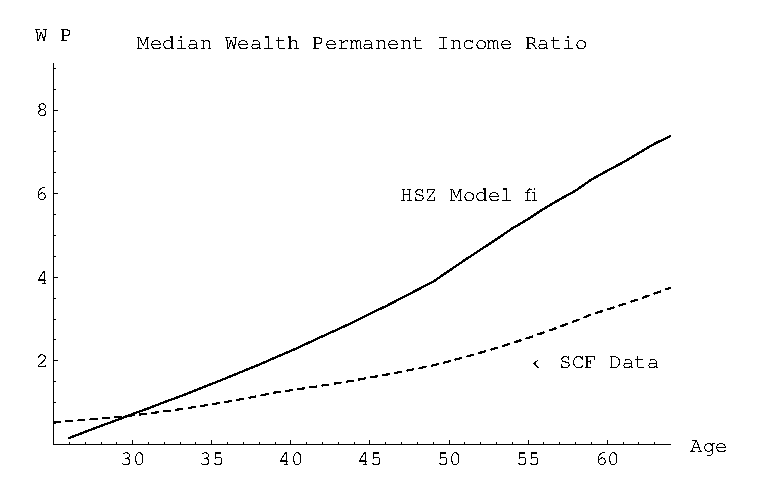
\includegraphics{./Figures/MedianWProfilesHSZvsSCF}}
	\caption{Median Wealth to Permanent Income Ratio, HSZ Model}
	\label{fig:MedianWProfilesHSZvsSCF}
\end{figure}


How, then, can the HSZ model produce overall averages that resemble 
the means of the SCF data?  The answer lies in the wealth holdings of 
the top few percent of the distribution.  The solid line in 
figure~\ref{fig:Top1pctWProfilesHSZvsSCF} shows, for each age group, 
the average ratio of wealth to permanent income for households at the 
99th percentile (by age) in the HSZ model.  The dashing line shows the 
corresponding calculation using the actual data from the 1992 and 1995 
SCFs.  Clearly, the richest SCF households own enormously more wealth, 
in relation to their permanent income, than the richest consumers in 
the HSZ model.

\hypertarget{Top1pctWProfilesHSZvsSCF}{}
\ifthenelse{\boolean{Figures}}{
\begin{figure}[p]
	\centerline{\includegraphics{./Figures/Top1pctWProfilesHSZvsSCF}}
	\caption{99th Percentile of Wealth to Permanent Income Ratio, HSZ Model}
	\protect\label{fig:Top1pctWProfilesHSZvsSCF}
\end{figure}
}

Taken together, Figures~\ref{fig:MedianWProfilesHSZvsSCF} and 
~\ref{fig:Top1pctWProfilesHSZvsSCF} show that the stochastic Life 
Cycle model under HSZ parameter values matches the aggregate and 
average data only because it makes two offsetting errors: 
overestimating the wealth of the typical household and underestimating 
the wealth of the richest households.

These simulations indicate that even the extended Life Cycle model 
misses some crucial features of household behavior.  However, the 
model's overprediction of the wealth of the median household is easily 
rectified; Carroll~\citeyear{carroll:brookings,carrollBSLCPIH} argues 
that the model captures the main features of the behavior of the 
median household very well if consumers are assumed to be slightly more 
impatient than HSZ assume, and if the income process is modified to 
include the benefits of aggregate productivity growth (HSZ assume that 
households expect, and experience, zero aggregate productivity growth 
over their lifetimes).  

If assuming that consumers are somewhat more impatient can make the 
stochastic Life Cycle model match the behavior of the median 
household, a natural question is whether assuming that consumers are 
somewhat more {\it patient} can make the model match the richest 
households.  If so, then it might be possible to argue that the only 
modification needed to make the stochastic Life Cycle model match the 
facts is to assume that consumers with higher lifetime incomes are 
also more patient.  Figure~\ref{fig:Top1pctWProfilePatientvsSCF} 
examines this possibility by showing the pattern of wealth over the 
working life of consumers who are the same as the consumers in the 
baseline HSZ model except that they have a time preference rate of 
zero rather than the baseline HSZ time preference rate of 3 percent 
annually.  While the age/wealth profile is certainly higher than in 
the standard HSZ model, it remains far below the profile for 
the consumers in the top 1 percent of the SCF data.  Plausible 
modifications of other parameter values also fail to raise the model 
profile to the level found in the data.  In other words, the richest 
households are saving more than can be justified even in a version of 
the Life Cycle model that allows for very patient consumers with a 
strong precautionary saving motive.

\hypertarget{Top1pctWProfilePatientvsSCF}{}
\ifthenelse{\boolean{Figures}}{
\begin{figure}[tbp]
	\centerline{\includegraphics{./Figures/Top1pctWProfilePatientvsSCF}}
	\caption{Wealth Profiles for Baseline and More Patient Consumers}
	\protect\label{fig:Top1pctWProfilePatientvsSCF}
\end{figure}}

The evidence presented thus far has concerned the saving behavior and 
wealth profiles of consumers during the working period of life.  The 
Life Cycle model has another set of testable implications for behavior 
in the latter stages of life, after retirement.  In particular, 
according to the standard Life Cycle model, even patient consumers 
want to spend all of their wealth before they die.  Of course, an 
uncertain date of death makes this difficult to achieve on one's own.  
However, there is a financial instrument which accomplishes exactly 
the goal implied by the model: annuities.  One test of the rough 
accuracy of the basic Life Cycle model is therefore whether the wealth 
of retired households is largely annuitized.

Carrying out such a test requires some methodology for calculating 
annuity wealth.  I assume that the annuity is fixed in real terms 
(primarily because the largest form of annuity income, Social 
Security, is inflation-adjusted).  I assume a real interest rate, and 
use the mortality tables from HSZ to construct the expected present 
discounted value of a one-dollar per year annuity as:
\begin{equation}
\Gamma_{a} = \sum_{i=a}^{T} \left(\prod_{j=a}^{i} \Lambda_{j}\right) R^{a-i},
\end{equation}
where $\Lambda_{i}$ is the probability of surviving from year $i-1$ to 
year $i$ and $R=1+r$ is the gross interest rate (I assume $R=1.03$ but 
results would be similar for other plausible interest rates).  The 
wealth value of the observed annuity income YANN at age a is then 
$\Gamma_{a}$ YANN$_{a}$.

Using this method, and including home equity among annuitized wealth, 
the mean household over age 65 has approximately 55 percent of their 
wealth in annuitized form.  However, among the richest 1 percent of 
households, the mean annuitization rate is only 10 percent.  

This evidence on annuitization is suggestive, but hardly conclusive.  
Annuity markets are likely far from perfect; as in other insurance 
markets, adverse selection may distort the market sufficiently to make 
inference hazardous.  Furthermore, annuities are the perfect financial 
vehicle to counter only one kind of risk, mortality risk.  If other 
kinds of risk are important, it is no longer obvious that even selfish 
Life Cycle consumers should annuitize most or all of their wealth.  
For example, if there is a small probability of a very expensive 
medical problem, it may be important to have access to a large chunk 
of nonannuitized wealth in order to pay the bills (assuming that no 
health insurance will fully cover every possible medical catastrophe 
or every potentially desirable experimental treatment).

An extreme assumption would be that annuity markets are so imperfect 
that, for practical purposes, we can assume that annuities cannot be 
purchased.  This assumption would obviously vitiate the argument that 
the failure of the wealthy to annuitize their wealth proves that they 
are not Life Cyclers.  However, in the absence of annuities the Life 
Cycle model has other implications.  In particular, it implies that 
selfish Life Cycle consumers, even patient ones, will eventually begin 
running down their wealth as they age.  Figure~\ref{fig:WealthFalls} 
shows that by age 80 or so the HSZ model implies that consumers should 
be dissaving at a fairly substantial pace (the simulations here follow 
HSZ's assumptions about mortality rates, which they derived from 
actuarial data, with the modification that they assume that death 
occurs for certain at age 100 if it hasn't happened yet).  However, 
Figure~\ref{fig:OldRichDontDissave} shows the actual average age 
profile of wealth across the four SCF surveys.  Although wealth 
accumulation slows, or perhaps halts, around age 65, there is no 
noticeable decumulation of assets for consumers in the top percentile 
of the wealth distribution.\footnote{The methods for construcing this 
figure draw on a literature dating at least to Browning, Deaton, and 
Irish~\citeyear{bdiProfitable} and with recent contributions by Attanasio 
and Weber~\citeyear{aw95}.  These authors have shown how to 
construct `synthetic panels' from a series of cross-section surveys 
like the four SCFs used in this paper.  That literature has noted that 
age, time, and cohort effects cannot be independently distinguished 
using such data, because age, time, and cohort are linearly related. 
The assumptions I made to identify age effects were, first, that 
cohort effects can be captured by a single term reflecting the 
lifetime level of permanent income of each cohort, (which I assume 
increased on average by 1.5 percent per annum for the cohorts in 
question, if anything an underestimate of the relevant average 
productivity growth rate and therefore a source of downward bias in 
the slope of the estimated age profile); and, second, that the time 
effects averaged to zero over the four SCF surveys.}

\hypertarget{WealthFalls}{}
\ifthenelse{\boolean{Figures}}{
\begin{figure}[p]
	\centerline{\includegraphics{./Figures/WealthFalls}}
	\caption{Age Profile of Log Wealth for the 99th Percentile, HSZ Model}
	\protect\label{fig:WealthFalls}
\end{figure}
}

\hypertarget{OldRichDontDissave}{}
\ifthenelse{\boolean{Figures}}{
\begin{figure}[p]
	\centerline{\includegraphics{./Figures/OldRichDontDissave}}
	\caption{Age Profile of Log Wealth for the 99th Percentile, SCF Data}
	\protect\label{fig:OldRichDontDissave}
\end{figure}
}

Of course, nothing in economics requires us to believe that the only 
purpose of saving is to finance one's own future consumption; that is 
merely a hypothesis of the basic Life Cycle model.  One natural idea is 
that the wealthy do not run down their assets because they want to 
leave bequests to their children.  This thought leads to the next model.

\medskip
\begin{quote}
``I would as soon leave my son a curse as the almighty dollar.''
~~\emph{Andrew Carnegie.}
\end{quote}

\hypertarget{the-dynastic-model}{}
\section{The Dynastic Model}
\label{sec:DynastyModel}

In the 1995 issue of the annual {\it Forbes 400} count of the richest 
Americans, there are at least 11 households containing descendants of 
Pierre du Pont (died 1817).  This might seem to be compelling evidence 
that at least some of the very rich have a powerful bequest motive.  
On the other hand, apparently no members of the 400 trace their wealth 
to Robert Morris, reputed to be the wealthiest man in America at the 
time of the Revolutionary War.  And Andrew Carnegie gave away over 90 
percent of his fortune before he died.  Furthermore, the fact that 
large bequests to children do occur does not prove that provision of 
such bequests is the primary motivation for accumulation.  

This section of the paper considers a particular model of bequests 
proposed by Barro~\citeyear{barro:bondsnetworth}.  The dynast alive at 
time $t$ is assumed to solve the intertemporal maximization 
problem:

\begin{eqnarray}
 	\max_{C_{t}} & U(C_{t}) + \displaystyle \sum_{i=t+1}^{\infty} 
 	\beta^{i-t} U(C_{i}) \\
 	\mbox{s.t.} & W_{t+1} = R[W_{t} - C_{t}] + Y_{t+1}, \nonumber
	\label{eq:dynasty}
\end{eqnarray}

where $C_{t}$ corresponds to the lifetime consumption spending of the 
generation living at time $t$, $W$ is the dynasty's wealth, $Y$ is the 
(noncapital) income earned by that generation, $R$ is the 
intergenerational interest rate, and $\beta$ is the discount factor.  
The implications of this equation for macroeconomics spawned the large 
literature on Ricardian equivalence in the 1970s and 1980s.  More 
recently, Altonji, Hayashi and Kotlikoff~\citeyear{ahk:altruism} have 
tested the Dynastic model with household-level data from the {\it 
Panel Study of Income Dynamics} and rejected its strong implication 
that only dynastic resources should matter for any individual family's 
consumption.  The typical PSID family, however, is not particularly 
wealthy, so those results do not necessarily imply that the Dynastic 
model is a poor one for the wealthiest families.

Although intuition suggests that the dynastic model might be 
interchangable with other models in which leaving a bequest yields 
utility, in fact the model has distinctive implications, such as 
Ricardian equivalence, that need not follow from other models of 
bequests.  As a result, the economic literature has drawn a 
distinction between Dynastic models like the one specified in 
equation~\ref{eq:dynasty} and ``Joy of Giving'' models in which the 
bequest yields utility directly.  For example, the Dynastic model 
implies that the size of the bequest should be a function of the ratio 
of the parent's lifetime income and the child's lifetime income; that 
parents should give larger bequests to poorer children; and that 
childless wealthy people should leave no bequests.  All of these 
implications of the Dynastic model have been tested in 
population-representative datasets and none has received consistent 
empirical support.  This section provides evidence that the Dynastic 
model is also a poor description of the behavior of the richest 
households.

To begin with some very informal evidence, Kennickell, Starr-McCluer, 
and Sunden~\citeyear{scf:focusgroup} report some results from a ``focus 
group'' session on saving motivations that was convened as part of the 
preliminary work in designing the questions for the 1995 
SCF.\footnote{Focus groups are commonly used in the preliminary stages 
of survey design to test sample questions and to explore whether 
respondents interpret questions in the intended way; to identify 
plausible ranges of behavior that might be exhibited by survey 
respondents; and for suggesting the most important sources of 
variation across individuals.} The eight members of the group were all 
wealthy individuals,\footnote{They were required to have a minimum 
annual income of \$250,000, minimum net worth of \$600,000, or both.} 
mostly in their 50s.  Participants were asked ``Thinking about your 
reasons for saving, what sorts of reasons are most important to you?''  
In the entire course of a three hour conversation of saving behavior, 
however, providing a bequest was not mentioned once as a reason for 
saving.\footnote{The only remark even tangentially related to 
inheritance was one woman's comment: ``When I die, my daughter's 
reaction is going to be, `Mother's dead?  That's too bad.  WHERE'S THE 
JEWELRY?'''}

A group of eight individuals is obviously too small a sample to 
convincingly demonstrate the general absence of a bequest motive among 
the wealthy.  Somewhat more persuasive evidence is provided in the 
results of survey questions on the 1992 SCF. Respondents were asked to 
list their five most important reasons for saving.  As shown in 
Table~\ref{table:DoRichSaveForKids}, only three percent of the general 
population, and two percent of the wealthy households, indicated that 
providing an inheritance was the most important reason to 
save.~\footnote{A similar question was asked in the 1995 SCF, with 
similar results.} Furthermore, only 5 percent of the total population 
and 4 percent of the wealthy households indicated that providing an 
inheritance was among their {\it top 5} reasons for saving.  (The 
differences between the wealthy households and the general population 
are not statistically significant here.)

\hypertarget{DoRichSaveForKids}{}
\begin{table}[tbp]
\center
\begin{tabular}{lccr}
	             &  Most     &  One of the 5      & Number \\ 
  	             & Important &  Most Important &    of    \\
   	             & Reason    &  Reasons          & Observations \\ \hline
Entire Sample    &  .03      &  .05              & 3254 \\
Richest 1 Percent & .02      &  .04              & 652 \\ \hline
\end{tabular}
	\caption{Percent Saying Inheritance is Important Reason to Save}
	\protect\label{table:DoRichSaveForKids}
\end{table}


Another obvious test of the model is to see whether the childless 
elderly tend to dissave more than those with children.  This 
hypothesis has been tested using population-representative data; 
Hurd~\citeyear{hurd:bequests} found that in the population as a whole, 
there is no tendency for elderly with children to decumulate faster 
than those without.  Unfortunately, even when the data from the four 
SCFs are combined, the number of childless, elderly, wealthy 
households is too small to permit reliable estimation of age profiles 
of wealth (only about ten percent of elderly couples are childless).

Another option is to consider what childless elderly people 
say about their saving and spending behavior.  Respondents to the 1992 
and 1995 SCFs were asked whether their spending was greater than, 
equal to, or less than their income over the past year, and how 
spending usually compared with income.  The results are presented in 
Table~\ref{table:SavOfRichOldByKidStatus}.\footnote{There is a strong 
correlation between the level of net worth and the answer to these 
questions.  The median net worth of consumers who said their 
consumption regularly exceeded their income was \$47,599; that of 
consumers who said their consumption did not usually exceed their 
income was \$154,079.} The childless elderly were {\it less} likely to 
say that they dissave than those with children, by this crude measure, 
either as a general rule or in the current year in particular.  Of 
course, it is possible that some of the ``spending'' of the elderly 
with children consists of {\it inter vivos} transfers to those 
children.  The real problem for the Life Cycle model is the testimony 
of the childless, wealthy elderly, essentially none of whom say that 
their spending exceeds their income.  This is all the more impressive 
given the comparatively small fraction of their income that is 
annuitized.
\hypertarget{saving-by-the-wealthy-elderly-with-and-without-children}{}
\begin{table}[tbp]
\center
\begin{tabular}[c]{lccc}
          & Spending  & Spending  \\ 
  	      &  Usually   & Exceeded  \\
   	      &  Exceeds   & Income    \\
   	      &  Income    & this year \\ \hline
With kids &  .05    & .23       \\ 
No kids   &  .00    & .00       \\ \hline
\end{tabular}
	\caption{Saving By the Wealthy Elderly With and Without Children}
	\protect\label{table:SavOfRichOldByKidStatus}
\end{table}
%\afterpage{\clearpage}

Given the paucity of publicly available data on the very wealthy, it 
is not surprising that the economic literature contains almost no 
empirical studies that shed any light on the behavior of the childless 
wealthy elderly (although there have been several studies that have 
examined the behavior of {\it non-wealthy} childless elderly 
households, and have found that they do not dissave; see, e.g., 
Menchik and David~\citeyear{menchik&david:nodissav} and the references 
therein).  I was able to find only one study that contains even 
tangential information on the subject, a paper by Auten and 
Joulfaian~\citeyear{auten&joulfaian:charitable} which uses a proprietary 
dataset compiled by the Internal Revenue Service on 1982 decedents who 
paid estate taxes.  From figures in their Table 1, p.  62 it is 
possible to calculate that the mean wealth of the childless decedents 
was virtually identical to that of those with children - hardly what 
would be expected if those with children had a powerful dynastic 
saving motive which the childless (presumably) do not 
share.\footnote{Of course, one might argue that the `dynasty' of the 
childless couples could be carried on by nephews and nieces, or second 
cousins, or any other heir who might be found.  However, such an 
argument only intensifies the problems with the dynastic model pointed 
out by Bagwell and Bernheim~\citeyear{bagwell&bernheim:sex}, to wit, that 
sexual reproduction and non-perfectly-assortative mating imply that 
eventually one's own descendants are so intermixed with everyone 
else's that there is no plausible sense in which a `dynasty' can be 
said to exist at all.} Furthermore, those {\it with} children actually 
contributed slightly {\it more} to charity during their lifetimes than 
the childless.  Again, a dynastic motive would suggest the opposite.  
Finally, Auten and Joulfaian found no significant effect of children's 
income on the size of charitable bequests.  This finding is consistent 
with evidence by Wilhelm~\citeyear{wilhelm:bequest} who found little 
support for the altruism model's implication that the size of bequests 
in families with more than one child should be related to the relative 
lifetime income of the children.  Instead, Wilhelm found roughly equal 
bequests in about 80 percent of bequests.

\hypertarget{the-capitalist-spirit}{}
\section{The Capitalist Spirit}
\label{sec:CapitalistModel}

This section presents a model in which wealth enters consumers' 
utility functions directly, and argues that such a model is both 
consistent with the available data on the saving behavior of the 
wealthy and plausible on grounds other than its consistency with 
these facts.  Zou~\citeyear{zou:spirit} and Bakshi and 
Chen~\citeyear{bakshi&chen:spirit} have recently noted that Max 
Weber~\citeyear{weber:capitalism} long ago argued that the pursuit of 
wealth for its own sake was the `spirit of capitalism,' and so I will 
call this the `Capitalist Spirit' model.

\hypertarget{the-model}{}
\subsection{The Model}
\label{subsec:CapitalistModel}

Consider a consumer with lifetime wealth $w_{T}$.  Suppose the utility 
function for lifetime consumption is a standard CRRA utility function, 
$u(c_{t}) = \frac{c^{1-\rho}}{1-\rho}$, and suppose the consumer also 
obtains utility from wealth in a modified Stone-Geary form,
$$
  v(w_{t}) = \frac{(w + \gamma)^{1-\alpha}}{1-\alpha} \notag
$$

Formally, the consumer's maximization problem is:
\begin{eqnarray}
 	\max_{c_{t}} & u(c_{T}) + v(w_{T+1}) \\ \nonumber
  	           & \mbox{s.t.} w_{T+1} = w_{T} - c_{T}.  \nonumber
	\label{eq:LastPeriodProb}
\end{eqnarray}
The problem as described thus far can be interpreted in either of two 
ways.  The first interpretation is that the model describes a consumer 
deciding how to allocate lifetime resources between consumption and 
wealth, with wealth yielding utility directly.  The second 
interpretation is of a consumer deciding how to allocate lifetime 
resources between lifetime consumption and end-of-lifetime wealth.  
(The reasons end-of-period wealth might yield utility include the ``Joy 
of Giving'' bequest motive mentioned above, and several others.  See 
below for further discussion).  

\hypertarget{first-order-condition}{}
The first order condition for an interior solution to this problem is:
\begin{eqnarray}
 	u'(c_{T})    & = & v'(w_{T+1}) \\ \nonumber
 	c_{T}^{-\rho} & = & (w_{T} - c_{T} + \gamma)^{-\alpha}. \nonumber
	\label{eq:LastPeriodEuler}
\end{eqnarray}
Call the $c_{T}$ which satisfies this equation $c_{T}^{*}$.  It is 
clear that for sufficiently small $w_{T}$ the 
equation will be satisfied only by choosing a $c^{*}_{T}$ larger than 
$w_{T}$, that is, by ending with negative wealth.  If we impose the 
condition that consumers may not die in debt, the solution to the 
problem is:
\begin{eqnarray}
 	c_{T} = \mbox{Min}[c^{*}_{T}, w_{T}]  \nonumber
	\label{eq:LastPeriodSoln}
\end{eqnarray}
If $\rho > \alpha$, end-of-period wealth will be a luxury good.  Furthermore, 
if $\gamma$ is positive, there will be a range of initial wealth such 
that the marginal value of an extra dollar of consumption always 
exceeds the marginal value of an additional dollar of wealth.  In this 
range, the consumer will choose to spend all available resources and 
end the period (and life) with zero wealth.

The problem can be solved analytically if we choose $\rho = 2$ and 
$\alpha = 1$.  If we set $\gamma=1$ the solution is
\begin{eqnarray}
    c_{T}=\mbox{Min}[ {{-1 + {\sqrt{1 + 4\,\left( 1 + {\it w_{T}} \right) }}}\over 2}  ,w_{T}].
	\label{eq:GraphSoln}
\end{eqnarray}
Define the saving rate as the fraction of beginning-of-period total 
assets the consumer ends up holding at the end of the period, 
$w_{T+1}/w_{T}$.  Figure~\ref{fig:WIUFSave} shows the saving rate of 
this consumer as initial wealth goes from 0 to 10.  For initial wealth 
between 0 and 1 the consumer saves nothing, but above initial wealth 
of 1 the saving rate rises monotonically.  Furthermore, as $w_{T} 
\rightarrow \infty$ the saving rate approaches 100 percent.  

\hypertarget{WIUFSave}{}
\ifthenelse{\boolean{Figures}}{
\begin{figure}[tbp]
	\centerline{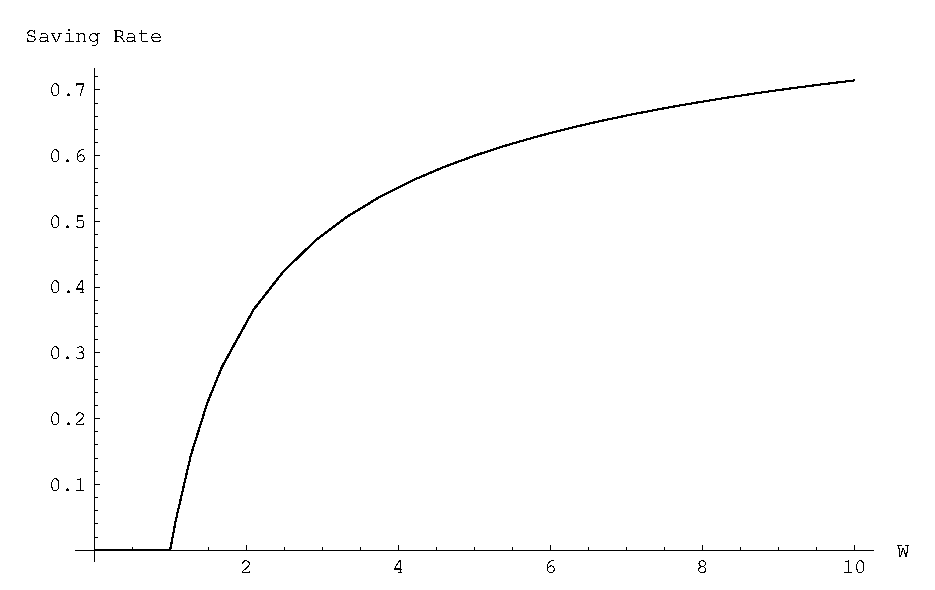
\includegraphics{./Figures/WIUFSave}}
	\caption{Saving as a Function of Wealth in the Capitalist Spirit Model}
	\protect\label{fig:WIUFSave}
\end{figure}
}

The essential insights from this model carry over when the model is 
extended to many periods and when labor and capital income are 
incorporated: consumers with permanent income below a certain 
threshhold will behave like standard Life Cyle consumers and will try 
to spend all their assets before death, while consumers with permanent 
incomes above the threshhold will save at ever increasing rates as 
lifetime income rises.

The idea that bequests (charitable or otherwise) are insignificant for 
most of the population, but become increasingly important in the upper 
reaches of the lifetime income distribution, has been informally 
expressed by several previous authors.  Indeed, 
Modigliani~\citeyear{modigliani:nobel} himself has argued that, to the 
extent that bequests must be included in the Life Cycle framework, 
they should be incorporated in precisely this ``luxury good'' manner.  
There is also a growing body of empirical evidence in support 
of the proposition.  Dynan, Skinner, and Zeldes~\citeyear{dsz:richsave} 
examine data from several micro datasets and find consistent and 
strong evidence that households with higher lifetime income leave 
larger bequests; Lillard and Karoly~\citeyear{lillard&karoly:richsave} 
find similar results.

In theoretical terms, the value added in this paper relative to the 
previous literature is simply the proposal of a specific and simple 
functional form for the consumer's utility function which captures the 
informal idea that rich people save more in a way that is at least 
roughly consistent with the empirical evidence marshalled above.  But 
such consistency may not be a high enough standard.

\begin{quote}
``Utility maximization is a metaphysical concept of impregnable 
circularity.''~~\emph{Joan Robinson~\citeyear{robinson:philosophy}, Economic 
Philosophy, Ch. 3.}
\end{quote}

\hypertarget{informal-evidence}{}
\subsection{Informal Evidence}
\label{subsec:InformalEv}
The essence of Joan Robinson's complaint about utility theory was that 
it is possible to construct a utility function to justify any 
conceivable behavior: Just assume that the behavior in question yields 
more utility than its alternatives.  Any postulated utility function, 
or proposed modification to a standard utility function, should 
therefore be defensible on grounds other than its ability to match the 
facts it was created to match.  This section argues, using a variety 
of informal evidence, that most qualitative descriptions of the 
behavior of the wealthy, both by the wealthy themselves and by outside 
observers, can be interpreted at a fundamental level as implying that 
wealthy people derive utility either directly from the ownership of 
wealth or indirectly, either from the activities that lead to wealth 
accumulation or from a flow of services that is closely tied to the 
ownership of that wealth.

The first important argument about the plausibility of the Capitalist 
Spirit model concerns the assumption that the marginal utility of 
consumption decreases sharply with the level of consumption.  What 
matters critically here is really the assumption that there is an 
alternative way to employ wealth whose marginal utility decreases more 
slowly than that of consumption (and hence will be a luxury good 
relative to consumption).  It is important to recall that the kind of 
consumption treated in the model is for strictly nondurable goods and 
services.  Carroll and Inhaber~\citeyear{scarrollHowRich} note that 
``luxury'' goods that are generally associated with the wealthy such 
as art, estates, jewelry -- even sports teams -- are almost all 
assets.  Indeed, beyond a certain level of wealth it becomes difficult 
to imagine how one could spend even the earnings on one's wealth on 
nondurable goods and services for personal enjoyment.  For example, 
recent press accounts have estimated Bill Gates's net worth at \$40 
billion.  Assuming a ten percent annual rate of return, Gates would 
have to spend \$4 billion a year, or over \$10 million a day, on 
nondurable goods and services simply to avoid further accumulation.

The proposition that the marginal utility of consumption approaches 
zero as the level of consumption rises is also lent credence by 
statements of wealthy people themselves.  Andrew Carnegie, Cornelius 
Vanderbilt, and other fabulously wealthy people refer to their 
``surplus'' wealth, and of determining when one has ``enough'' wealth.  
H.L. Hunt, then the richest man in the world, once said that ``for 
practical purposes, someone who has \$200,000 a year is as well off as 
I am.''  Similar statements (appropriately adjusted for inflation) 
have been attributed to William Henry Vanderbilt and John Jacob Astor, 
two 19th century plutocrats.

One of the appealing features of the idea that rich people eventually 
reach near-satiation in their consumption of nondurables is that this 
means one need not assume a towering and obsessive greed lies behind 
their continuing accumulation.  If `greed' is defined as a desire to 
possess wealth for its own sake, even a modest amount of greed will 
suffice, so long as greed does not diminish with wealth as fast as the 
marginal utility diminishes with consumption.  Or, to put the idea 
more concretely, if ownership of extra houses, yachts, artwork, or, 
for that matter, corporations has even a modest intrinsic appeal, 
eventually that appeal is likely to exceed waning lure of an extra 
dollar of nondurable consumption.  Of course, this is merely another 
way of saying that ownership of these kinds of wealth yields utility 
directly, as the basic Capitalist Spirit model assumes.

Of course, towering and obsessive greed cannot always be ruled out.

\begin{quote}
``The point is that you can't be too greedy.''~~\emph{Donald 
Trump~\citeyear{trump:deal}, in 
{\it Trump: The Art of the Deal}, ch.  2.}

``Greed is good.''~~\emph{Ivan Boesky, in an address to business school 
students, University of California at Berkeley, 1987.}

``The one with the most toys when he dies, wins.''~~\emph{Anonymous}
\end{quote}

And, among the 19th century plutocrats, according to historian 
Frederic Cople Jaher~\citeyear{jaher:gilded},
\begin{quote}
Money-making and keeping, not adorned or rationalized by nobler 
explanations, actually constituted a powerful force in the lives of 
the very rich.  As boys, [Mining magnate William Boyce] Thompson and 
[John D.] Rockefeller vowed to accumulate a fortune.  Thompson.\ldots 
and [Andrew] Carnegie promised themselves to retire after reaching a 
certain level of wealth, but kept pushing onward.  Rogers, a 
Rockefeller disciple and associate, said that the Standard Oil 
partners made the profit motive a `religion,' a faith `taught' them by 
`Mr.  Rockefeller.'
\end{quote}



To the extent that these quotations express the general truth about 
the motivations of the wealthy, the Capitalist Spirit model can be 
said to apply directly.  However, the view that all wealthy people are 
motivated solely by a love of wealth for its own sake is surely 
extreme.  A variety of other plausible, and apparently very different, 
motivations are commonly proposed, ranging from job satisfaction to 
status-seeking to philanthropic ambitions to power-lust.  The 
remainder of this section argues that, from a modelling standpoint, 
these other common ideas--different though they may be from a 
psychological perspective--are essentially indistinguishable from each 
other and from the basic Capitalist Spirit model in terms of their 
implications for individual behavior.  The argument, therefore, is 
that if {\it any} of these several proposed motivations is correct, 
the Capitalist Spirit model constitutes an appropriate mathematical 
model of the behavior of the wealthy.

Perhaps the most obvious example of a psychologically very different 
model which would be behaviorally indistinguishable from the 
wealth-in-the-utility-function model is the idea that the wealthy 
enjoy doing their jobs well, and that they view the accumulation of 
wealth as the principal measure of job performance.  This idea appears 
frequently both in the statements of the wealthy themselves and in 
commentary by others on the behavior of the wealthy.  Two particularly 
direct statements are:

\begin{quote}
``The rich man's `duty,' such as it is, is not to society but to his art, and 
his art is making money.''~~\emph{Michael Lewis, {\it The New York Times 
Sunday Magazine, July 1995}}

``Money's just a way of keeping score.  It's the game that matters.''
~~\emph{H. L. Hunt, cited in Jaher~\citeyear{jaher:gilded}, p. 215}
\end{quote}

A closely related idea is suggested by the work of Robert 
Frank~\citeyear{frank:rightpond}, who has argued that an intrinsic 
component of human nature is a tendency to judge oneself by comparison 
with others.  If for some wealthy people wealth is the metric of 
comparison, the utility function should contain not the absolute level 
of their wealth but some function of the relationship of their wealth 
to that of others.  Bakshi and Chen~\citeyear{bakshi&chen:spirit}, Cole, 
Mailath, and Postlewaite~\citeyear{cmp:socialnorms}, and 
Zou~\citeyear{zou:spirit} have also argued that wealth matters because it 
is an index of social status.\footnote{There is also a growing 
literature exploring the consequences if the utility obtained from 
consumption depends on a comparison of consumption to a reference 
stock determined either by one's own past consumption (Carroll, 
Overland, and Weil~\citeyear{cow:habits}; Campbell and 
Cochrane~\citeyear{campbell&cochrane:force}; 
Constantinides~\citeyear{constantinidesHabits}) or the consumption of 
others (Abel~\citeyear{abel:aerhabits}; Carroll, Overland, and 
Weil~\citeyear{cow:envy}).} For practical purposes of analysis of 
household-level data, however, either of these ideas is virtually 
indistinguishable from the proposition that wealth enters the utility 
function directly, and both ideas should produce essentially identical 
results in a model of saving (although they might have different 
implications for optimal tax policy; see the discussion below and the 
paper by Frank in this volume).\footnote{One problem with the 
particular specifications of Bakshi and Chen~\citeyear{bakshi&chen:spirit} 
and Zou~\citeyear{zou:spirit} is that their specifications imply that 
consumers with zero wealth would have negative infinite utility.  
According to the SCFs, however, about ten percent of the population 
has zero or negative net worth.  Furthermore, their model does not 
necessarily predict that high lifetime income consumers will save more 
than those with low lifetime income.  Finally, there is a growing 
consensus that the standard Life Cycle model, with an appropriate 
treatment of uncertainty, does a fairly good job of describing the 
behavior of the typical household without any need for important 
direct effects of wealth on utility.  Only at the upper reaches of the 
wealth distribution does behavior unmistakably diverge from the 
model's predictions.}

It is also possible that wealthy people continue accumulating because 
greater wealth yields some other benefit that is more difficult to 
measure, such as power.  In particular, the view that wealth 
brings power is commonplace among both the wealthy themselves and 
observers of the wealthy.  (The idea that power is desirable appears 
to be taken for granted.)

\begin{quote}
``The ultimate gift of colossal wealth, at least for the founders of the 
richest families, was power.''~~\emph{Jaher~\citeyear{jaher:gilded}, p.  215}

``Money is the measuring rod of power.''~~\emph{Howard Hughes}

``'Twasn't the money we were after, 'twas the power.  We were all 
playing for power.  It was a great game.''~~\emph{James Stillman, Gilded 
Age financier, cited in Jaher~\citeyear{jaher:gilded}}

``If you give away the surplus [money], you give away the 
control.''~~\emph{Cornelius Vanderbilt, cited in 
Jaher~\citeyear{jaher:gilded}}

```Tis a sort of duty to be rich, that it may be in one's power to do 
good, riches being another word for power.''~~\emph{Lady Mary Wortley 
Montagu (1689-1762), English society figure, letter writer.  Letter, 
c.  24 Sept.  1714, to her husband, cited in Jaher~\citeyear{jaher:gilded}.}
\end{quote}

This last quotation raises a final idea that crops up frequently in 
the statements of the wealthy themselves: that the purpose of 
accumulating wealth is ultimately to enable the wealthy person to 
pursue philanthropic activities, or to establish institutions to carry 
out such activities.  While such an evidently self-serving 
interpretation should be subject to considerable skepticism, there are 
many prominent examples of philanthropy that bear out the proposition.  
The Ford Foundation, the Rockefeller Foundation, Carnegie-Mellon 
University, Duke University, Johns Hopkins University, the Getty 
museum, and a host of other prominent institutions owe either their 
existence or a substantial part of their endowments to the munificence 
of wealthy individuals (often, although not always, manifested through 
bequests).  Morally, socially, and psychologically this motivation for 
wealth accumulation is very different from pure greed.  However, if 
more wealth allows one to establish a larger foundation or endow more 
institutions, the implications for saving behavior are again virtually 
indistinguishable from the idea that wealth enters the utility 
function directly.

\hypertarget{wealth-and-taxes}{}
\section{Death and Taxes}
Assuming that the Capitalist Spirit model provides a roughly correct 
description of the behavior of wealthy households, a natural question 
to ask is what the model implies about the relationship between 
accumulation behavior and taxes.~\footnote{I should note here that the 
following analysis is really only correct for those interpretations of 
the model in which consumers care about the absolute level of wealth 
or consumption.  If, instead, utility from $w_{T+1}$ depends on how 
large one's own $w_{T+1}$ is compares to the $w_{T+1}'s$ of others, 
bequest taxes would likely have a much smaller effect than that 
discussed below.  For an analysis of related issues in income 
taxation, see the paper by Frank in this volume.} Returning to the 
parameterized version of the model in which $\rho = 2$ and $\alpha = 
\gamma = 1$, if bequests (or wealth) are taxed at rate $\tau$ then the 
equation for optimal consumption becomes:

\begin{eqnarray}
    c_{T}=\min [ {{-1 + {\sqrt{1 + 4(w+\gamma/(1-\tau))}}} \over 2},w_{T}].
	\label{eq:TaxSoln}
\end{eqnarray}


Figure~\ref{fig:BequestTaxes} shows the effect on consumption if 
bequest taxes are increased from 40 percent to 80 percent.  Consider 
first the curve labelled $\tau = .4$, which shows the optimal amount 
of consumption for consumers facing a 40 percent bequest tax if 
bequests are not constrained to be positive.  The actual consumption 
function, of course, is the minimum of the 45 degree line and this 
curve.  The point of intersection of this curve and the 45 degree 
line, labelled $\omega_{1}$, reveals the level of lifetime wealth at 
which consumers begin to leave positive bequests.

When the bequest tax is raised to 80 percent, the amount of 
consumption shifts up, as indicated in the curve labelled $\tau = 
.8$.  The point at which consumers begin leaving bequests, 
$\omega_{2}$, is substantially higher than when the tax rate was 40 
percent.  

Hence, it is useful to think of the effects of raising the bequest tax 
by considering three categories of consumers.  The first are those 
with lifetime wealth less than $\omega_{1}$.  They leave bequests 
under neither tax regime, so their behavior is unaffected by the tax 
increase.  The second region is those consumers with lifetime wealth 
between $\omega_{1}$ and $\omega_{2}$.  These are the consumers who 
would leave bequests if the bequest tax were only 40 percent, but 
prefer to consume all of their lifetime wealth when the bequest tax 
rises.  Finally, consumers with lifetime wealth greater than 
$\omega_{2}$ will leave bequests even when the bequest tax is 80 
percent.  However, at any level of lifetime wealth the size of the 
bequests they leave is reduced by an amount equal to the gap between 
the two consumption curves.  It is simple to show that as lifetime 
wealth goes to infinity the fraction of lifetime wealth bequeathed 
approaches 100 percent even with the higher bequest taxes.  This is 
the region of the model presumably corresponds best to the 
circumstances of fabulously wealthy people like Bill Gates.

\hypertarget{BequestTaxes}{}
\ifthenelse{\boolean{Figures}}{
\begin{figure}[p]
	\centerline{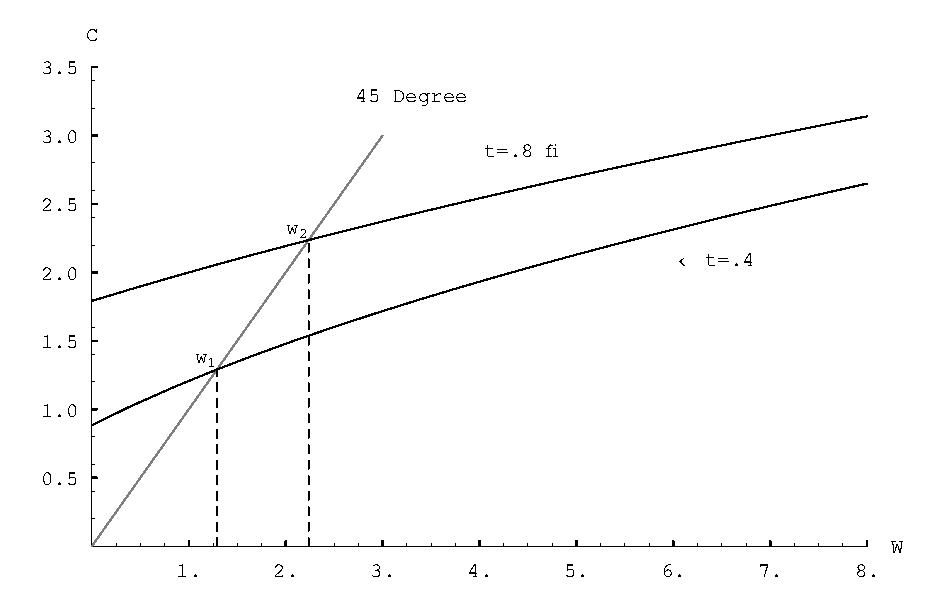
\includegraphics{./Figures/BequestTaxes}}
	\caption{Effect on Consumption of an Increase in Bequest Taxes}
	\protect\label{fig:BequestTaxes}
\end{figure}
}

%\afterpage{\clearpage}

Because the effect of taxes on consumption depends on the distribution 
of consumers across the different levels of lifetime income, the 
aggregate effect of bequest taxes in this model is impossible to judge 
in the absence of evidence (or assumptions) about the distribution of 
lifetime income (and information about the parameters of the model).  
If most bequests come from people with $\omega_{1} < w_{T} < 
\omega_{2}$, then an increase in the bequest tax could reduce bequests 
almost to nothing.  If, on the other hand, most bequeathed wealth 
comes from consumers with very large amounts of lifetime income, 
increasing the bequest tax might have very little effect on either 
consumption or (pre-tax) bequests.

In principle, it should be possible to tease out estimates of the 
relevant parameter values from available data on wealth, consumption 
and income, using methods like those employed in an impressive recent 
paper by Gourinchas and Parker~\citeyear{gpLifeCycle}.  
Those authors assume a ``residual value function'' that characterizes 
the utility experienced during the last part of life that is 
mathematically very similar to the ``bequest utility'' function 
postulated in the model here.  Gourinchas and Parker assume that the 
coefficient of relative risk aversion for the residual value function 
is the same as for the period utility function, and they do not 
incorporate a Stone-Geary term like my $\gamma$, but their estimation 
methodology could easily be adapted to estimate those two additional 
parameters.  Having estimated those parameters, they could then 
perform simulations to gauge the predicted impact of changes in 
bequest taxes on consumption.  

\hypertarget{conclusion}{}
\section{Conclusions}
A variety of evidence, both qualitative and quantitative, strongly 
suggests that people at the top end of the wealth and income 
distributions behave in ways that are substantially different from the 
behavior of most of the rest of the population.  In particular, it is 
difficult to explain the behavior of these consumers using the 
standard Life Cycle model of consumption.  A leading alternative to 
(or perhaps just an extension of) the Life Cycle model is the Dynastic 
model in which the decisionmaker cares about the utility of his 
descendants.  The Dynastic model, however, has problems of its own, 
starting with the testimony of many wealthy households who say that 
providing an inheritance is not a principal motivation for saving and 
ending with the fact that childless wealthy old people do not appear to 
dissave.  I argue that the simplest model capable of fitting all the 
facts is a model in which wealth either enters the utility function 
directly as a luxury good, or wealth yields a stream of services that 
enter the utility function in ways that would be formally virtually 
indistinguishable from a model in which wealth enters the utility 
function directly.

In a way, the model reconciles Fitzgerald and Hemingway.  Fitzgerald 
was right that rich do not behave simply as scaled-up versions of 
everyone else.  They choose to save more and to accumulate faster 
because they can ``afford'' the luxury of doing so.  But Hemingway was 
right to suggest that the rest of us would probably behave the same 
way, if only we had more money.

\vfill\clearpage\eject

\ifthenelse{\boolean{PublicationVersion}}{
   \newpage\begingroup
   \setlength{\parindent}{0pt}\setlength{\parskip}{3ex}
   \def\endnotesize{\normalsize}
   \theendnotes\endgroup
}


\vfill\clearpage
\baselineskip 18pt
\ifthenelse{\boolean{PublicationVersion}}{\baselineskip 30pt}

\bibliographystyle{plainnat}
\setcitestyle{authoryear}
\bibliography{economics,Why}

\vfill\eject


\end{document}
